


%-----------------------------------------------------------------------------------%
\documentclass[final]{beamer}
% Poster em modo retrato; ajuste o tamanho do banner aqui:
%   - size=a0  (A0 vertical)
%   - ou use size=custom,width=<cm>,height=<cm>
\usepackage[size=a0,orientation=portrait,scale=1.28]{beamerposter}
\renewcommand{\tablename}{Tabela}
\usepackage{subcaption} 
\usepackage{caption} 

% Define estilo ABNT para legendas de tabelas
\setbeamertemplate{caption}[numbered]
\captionsetup[table]{labelfont=bf, textfont=bf, justification=centering,
                     name=Tabela, labelsep=space, singlelinecheck=false}

% Pacotes essenciais
\usepackage{graphicx}
\usepackage{ragged2e}
\usepackage{array,booktabs}
\usepackage{tikz} 
\setlength{\parindent}{0pt}
\usepackage{listings}
\usepackage{xcolor}
\usepackage{minted} 


\lstset{
    language=Python,
    backgroundcolor=\color{backcolour},
    basicstyle=\ttfamily\small,
    keywordstyle=\color{blue}\bfseries,
    stringstyle=\color{red},
    commentstyle=\color{codegray},
    breaklines=true,
    showstringspaces=false,
    numbers=left,
    numberstyle=\tiny\color{gray},
    frame=single,
    captionpos=b
}

% Fundo em página inteira (suba "fundo.png" no projeto)
\usebackgroundtemplate{%
  
\includegraphics[width=\paperwidth,height=\paperheight]{fundoemr.png}%
}

% Cores e fontes simples (texto direto, sem "blocks" com caixa)
\setbeamercolor{normal text}{fg=black,bg=}
\setbeamerfont{title}{size=\huge,series=\bfseries}
\setbeamerfont{author}{size=\Large}
\setbeamerfont{institute}{size=\large}
\setbeamerfont{normal text}{size=\Large}


\begin{document}
\begin{frame}[t]



% ====== CABEÇALHO ======
\vspace*{7.0cm}
\centering
{\usebeamerfont{title} Comparação e Desempenhos dos Testes de Normalidade\\ 
  via Simulação de Monte Carlo em Linguagem R\par}
  
\vspace{0.8cm}
{\usebeamerfont{author} Mário Diego Rocha Valente (Graduando em Sistemas de Informação da UFPA)\par}

\vspace{0.8cm}
{\usebeamerfont{author} Breno Cauã Rodrigues da Silva (Graduando em Estatística da UFPA)\par}

\vspace{0.8cm}
{\usebeamerfont{author} Dennison Célio de Oliveira Carvalho (Prof. Dr., UFPA)\par}

\vspace{0.8cm}
{\usebeamerfont{author} Heliton Ribeiro Tavares (Prof. Dr., UFPA)\par}

{\usebeamerfont{institute}\texttt{Email:diego.valente@icen.ufpa.br, breno.silva@icen.ufpa.br, dennison@ufpa.br, heliton@ufpa.br  
}\par}
\vspace{3cm}

% ====== DUAS COLUNAS ======
\begin{columns}[t,totalwidth=0.6\paperwidth]
  % ----- Coluna Esquerda -----
  \hspace*{2.5cm}
  \begin{column}{0.45\paperwidth}


{\large\bfseries 1. INTRODUÇÃO}\par
\justifying
\vspace{1.3cm}

De modo geral, muitos métodos estatísticos requerem que os dados sigam uma distribuição normal e que as observações sejam independentes. Verificar a proximidade da distribuição dos dados com a normalidade torna-se, portanto, uma tarefa fundamental para garantir a validade desses métodos. Mas como podemos assegurar que a distribuição dos dados se aproxima de uma distribuição normal? Duas métricas primordiais para avaliar o desempenho dos testes de normalidade são as \textbf{Taxas de Erro Tipo I}, calculadas sob a hipótese nula ($H_0$), e o \textbf{Poder do Teste}, que é mensurado sob a hipótese alternativa ($H_1$). A análise dessas métricas permite identificar a capacidade de cada teste em evitar erros de falso positivo e, ao mesmo tempo, sua eficácia em detectar desvios de normalidade quando eles de fato existem (CARDOSO e FERREIRA, 2010).

\vspace{1.3cm}
{\large\bfseries 2. MATERIAIS E MÉTODOS}\par
\justifying
\vspace{1.3cm}

{\large\bfseries 2.1 Software}\par

Para conduzir as análises e estimativas neste estudo, foi utilizada a linguagem de programação \textbf{$R_{4.5.1}$}, empregando a IDE \href{https://posit.co/download/rstudio-desktop/}{\textit{\textbf{RStudio}}}, versão 1.12. Os seguintes pacotes foram utilizados nas diversas etapas do processo de simulação dos testes de normalidade: \textbf{DistributionTest} ,\textbf{irr}, \textbf{moments},\textbf{nortest}, \textbf{DescTools}.  

\vspace{1.3cm}
{\large\bfseries 2.2 Simulação de Monte Carlo}\par

Neste estudo, a eficácia dos testes de normalidade foi avaliada por meio da simulação de amostras tanto de distribuições normais quanto não normais, abrangendo casos simétricos e assimétricos, incluindo as distribuições Normal, Uniforme, Beta, t-Student, Cauchy e Exponencial. Foram considerados seis tamanhos amostrais distintos para cada distribuição: 30, 50, 100, 300,
500 e 1000. Em cada caso, foram realizadas 2.000 replicações, durante as quais os testes de normalidade foram registrados para análise posterior. Utilizou-se o teste Kappa de Fleiss, implementado pela função Kappam.fleiss() do pacote irr, com o objetivo de avaliar o nível de concordância entre os testes de normalidade.



 \vspace{1em}
{\large\bfseries 3. RESULTADOS E DISCUSSÃO}\par
\justifying
\vspace{1.3cm}

%Para reprodutibilidade deste estudo, o script em R foi armazenado em um repositório %no \textit{Github} que pode ser acessado no seguinte link: %\href{https://github.com/MarioDhiego/Teste\_Normalidade}{Testes de Normalidade}.

\vspace{0.5cm}

%Os resultados do Teste de Kappa-Fleiss estão dispostos na Tabela (\ref{tab:resultKappaFleiss}) para as Distribuições de Probabilidade $Normal(0, 1)$, %$Beta(2, 5)$ e $Cauchy(0, 1)$.

\begin{table}[H]
\centering
 \setlength{\tabcolsep}{8pt}
    \renewcommand{\arraystretch}{1.25}
\caption{Teste kappa-Fleiss de Concordância para os testes de normalidade.}
   \begin{tabular}{c|c}
\toprule
Distribuição de Probabilidade  &  Teste de Kappa-Fleiss \\
\midrule
$Normal(0, 1)$  &  0,93  \\
$Beta(2, 5)$    &  0,89  \\
$Cauchy(0, 1)$  &  0,81  \\
\bottomrule
\end{tabular}
    \label{tab:resultKappaFleiss}
\end{table}

%Percebe-se que para a maioria das distribuições, os testes tiveram forte concordância %entre rejeitar ou não a hipótese de normalidade. 

\vspace{0.5cm}

%A tabela (\ref{tab:inverted2}) apresenta os resultados obtidos da sensibilidade para cada teste e tamanho amostral.

\begin{table}[H]
    \centering
    \caption{Taxa de Acertos para a Sensibilidade dos Testes de Normalidade.}
    \begin{tabular}{c|c|c|c|c|c|c|c|c|c|c|c}
    \hline \hline
Distribuição              & Amostra &   AD  & CVM  &  DA   & JB   &  KS   & Lilli &  SW  & $Z_{A}$ & $Z_{C}$ & $Z_{K}$ \\
    \hline
\multirow{6}{*}{Beta (2,5)} 
                          & 30      & 1.0   & 0.82 & 0.81  & 0.87 &  1.0  &  0.85  &  0.75 &  0.73  & 0.76   & 0.81   \\
                          & 50      & 1.0   & 0.74 & 0.73  & 0.84 &  0.99 &  0.79  &  0.62 &  0.55  & 0.63   & 0.68   \\
                          & 100     & 0.99  & 0.51 & 0.47  & 0.70 &  0.98 &  0.62  &  0.27 &  0.17  & 0.27   & 0.28   \\
                          & 300     & 0.99  & 0.49 & 0.46  & 0.69 &  0.98 &  0.61  &  0.27 &  0.18  & 0.26   & 0.29    \\
                          & 500     & 0.28  & 0.003 & 0.001  & 0.002 & 0.49  & 0.02 & 0.01  & 0.01  & 0.01   & 0.01     \\
                          & 1000    & 0.004  & 0.10  & 0.010  & 0.10 & 0.10  & 0.10  & 0.10  & 0.10  & 0.10  & 0.10       \\
                          \hline\hline
\multirow{6}{*}{Normal (0,1)}   
                          & 30      & 1.0   & 0.95  & 0.94  & 0.93 &  1.0  &  0.95  & 0.94  &  0.94  &  0.94  & 0.95   \\
                          &  50     & 1.0   & 0.94  &  0.94 & 0.93 &  1.0  &  0.94  & 0.94  &  0.94  &  0.94  & 0.94    \\
                          & 100     & 1.0   &  0.95 &  0.95 & 0.93 &  1.0  &  0.95  & 0.95  &  0.94  &  9.94  & 0.94   \\
                          & 300     &       &       &       &      &       &        &       &        &        &        \\
                          & 500     &       &       &       &      &       &        &       &        &        &        \\
                          & 1000    &       &       &       &      &       &        &       &        &        &        \\  
                          \hline\hline
\multirow{6}{*}{Couchy (0,1)}     
                         & 30       &       &       &       &      &       &             &       &         &         &        \\
                         &  50      &       &       &       &      &       &             &       &         &         &        \\
                         & 100      &       &       &       &      &       &             &       &         &         &        \\
                         & 300      &       &       &       &      &       &             &       &         &         &        \\
                         & 500      &       &       &       &      &       &             &       &         &         &        \\
                         & 1000     &       &       &       &      &       &             &       &         &         &        \\
    \hline \hline
    \end{tabular}
    \label{tab:inverted2}
\end{table}


\vspace{1em}
 \justifying
 
  \end{column}
  \hspace{0.02\paperwidth} 
  %\hspace{1.5cm} % “gutter” entre as colunas — ajuste se quiser

  % ----- Coluna Direita -----
  \begin{column}{0.45\textwidth}
 
{\large\bfseries 4. SIMULAÇÃO IN R}\par
\justifying
\vspace{1.3cm}

{\large\bfseries 4.1 Script}\par
\vspace{1.3cm}

\begin{figure}[H]
    \centering
    % --- Primeira figura ---
    \begin{subfigure}[b]{0.32\linewidth}
        \centering
        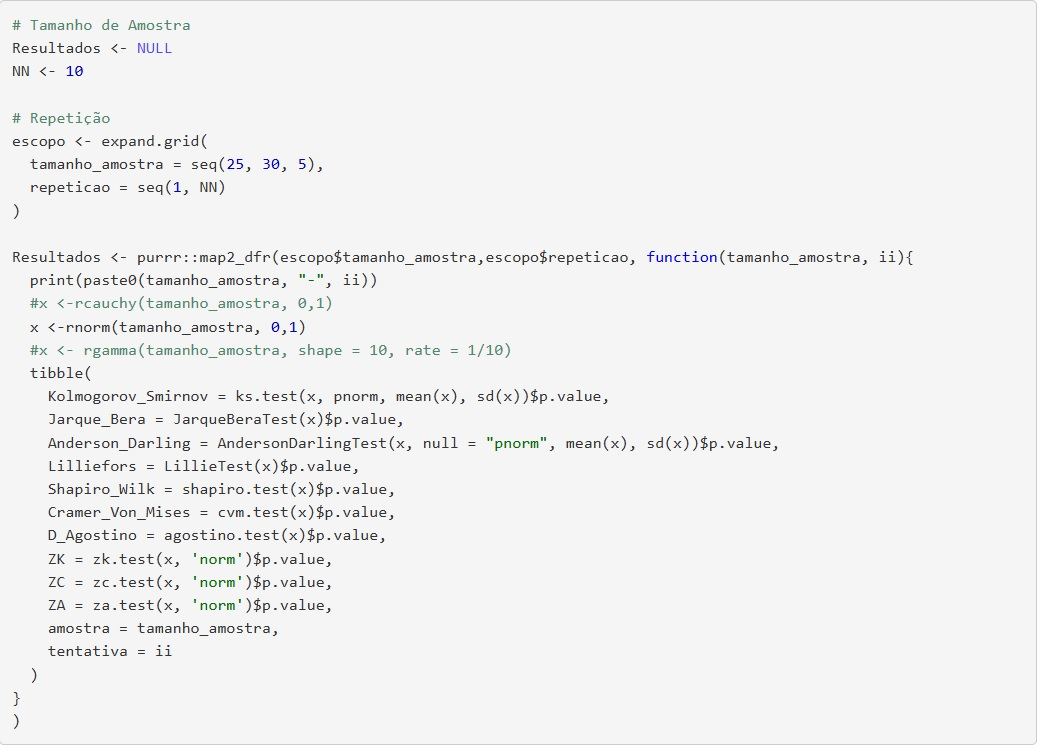
\includegraphics[width=\linewidth]{fig1_simulacao.jpg}
        \caption{Tamanho de Amostra}
        \label{fig:simulacao1}
    \end{subfigure}
    \hfill
    % --- Segunda figura ---
    \begin{subfigure}[b]{0.33\linewidth}
        \centering
        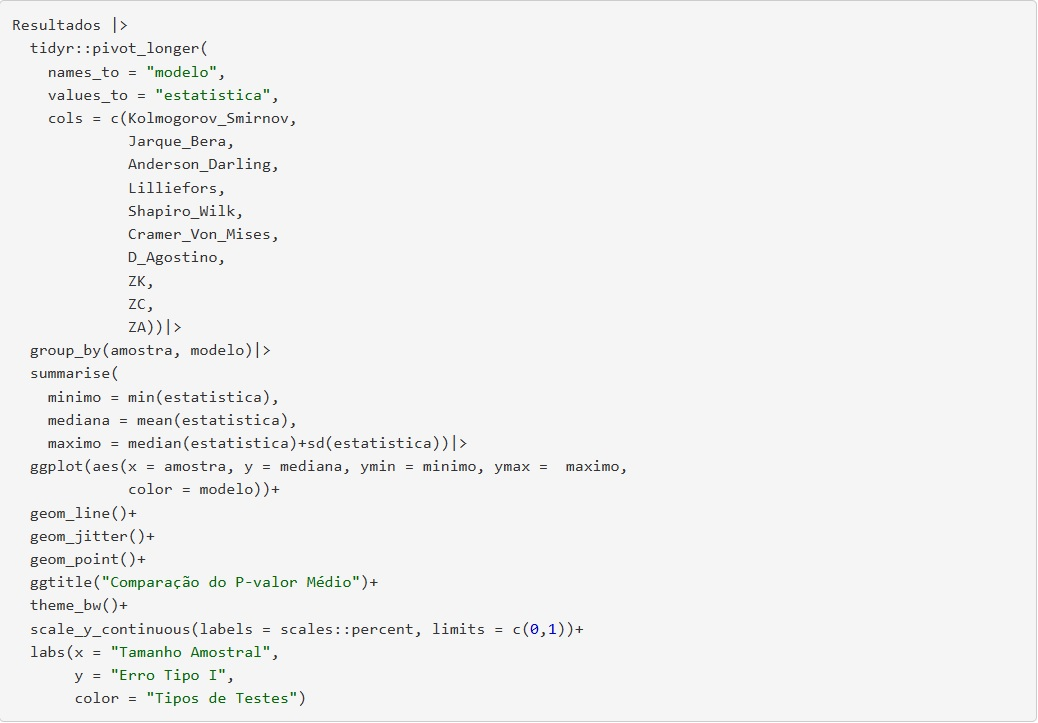
\includegraphics[width=\linewidth]{fig2_simulacao.jpg}
        \caption{Erro Tipo I (P-valor)}
        \label{fig:simulacao2}
    \end{subfigure}
    \hfill
    % --- Terceira figura ---
    \begin{subfigure}[b]{0.33\linewidth}
        \centering
        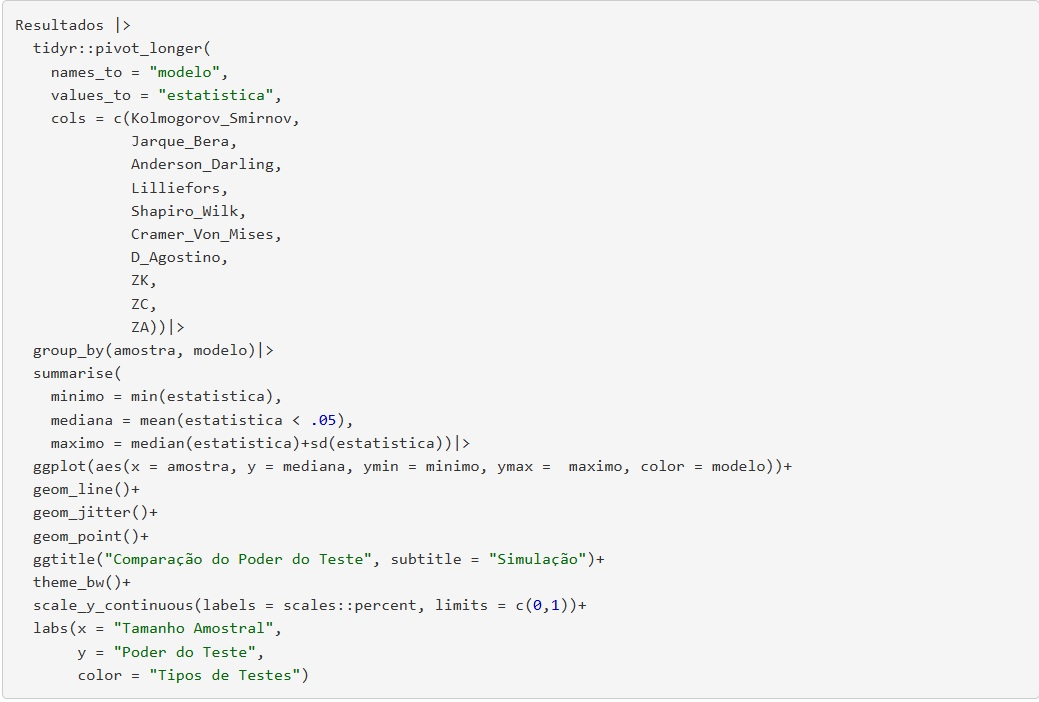
\includegraphics[width=\linewidth]{fig3_simulacao.jpg}
        \caption{Poder do Teste}
        \label{fig:simulacao3}
    \end{subfigure}

    \caption{Simulações em linguagem R: (a) Tamanho de amostra, (b) Erro Tipo I e (c) Terceira simulação.}
    \label{fig:simulacoes}
\end{figure}


%%%%%%%%%% Erro Tipo I -> Distribuição Beta %%%%%%%%%%
\begin{figure}[H]
    \centering
      \caption{Comparação do Erro Tipo I dos testes AD, CM, DG, LL, JB, KS, LL, ZA, ZC e ZK em função do tamanho amostral para a \textbf{Distribuição} $\textbf{Cauchy}(0, 1)$.}
    \label{fig:erro_tipo_I_dist_cauchy}
    % Primeira figura
    \begin{subfigure}[b]{0.3\textwidth}
        \centering
        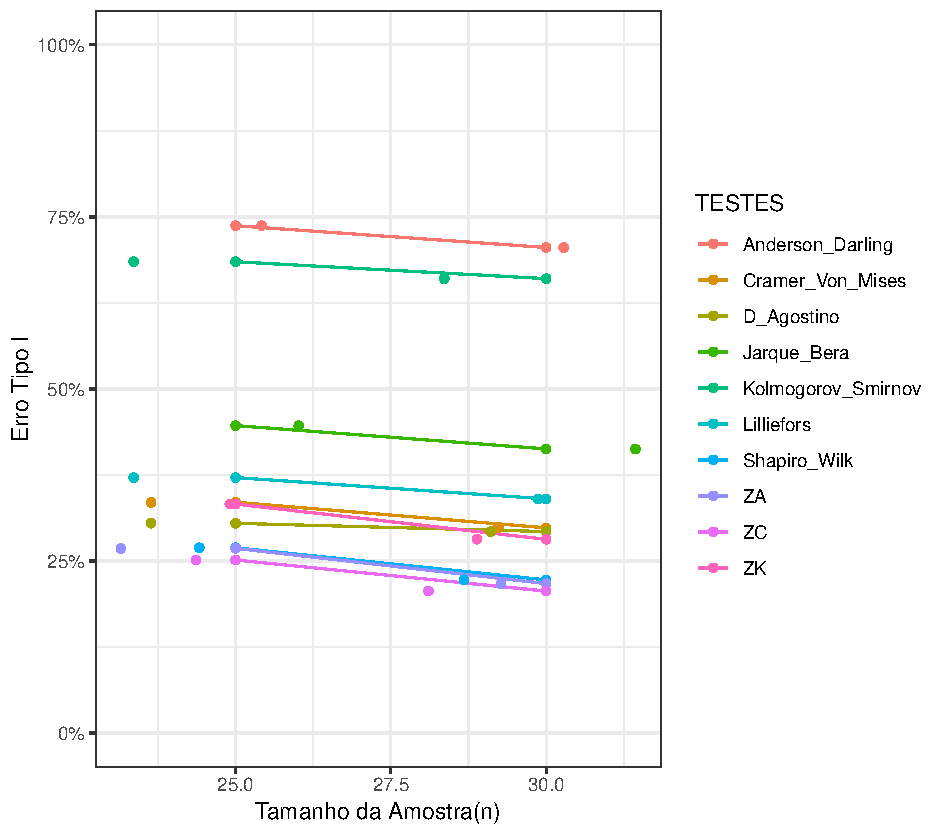
\includegraphics[width=\textwidth]{Distribuição_Beta/Erro_TipoI/erro_tipo_I_beta_30.pdf}
        \caption{(\(N = 30\)}
        \label{fig:beta_30}
    \end{subfigure}
    \hfill
    % Segunda figura
    \begin{subfigure}[b]{0.3\textwidth}
        \centering
        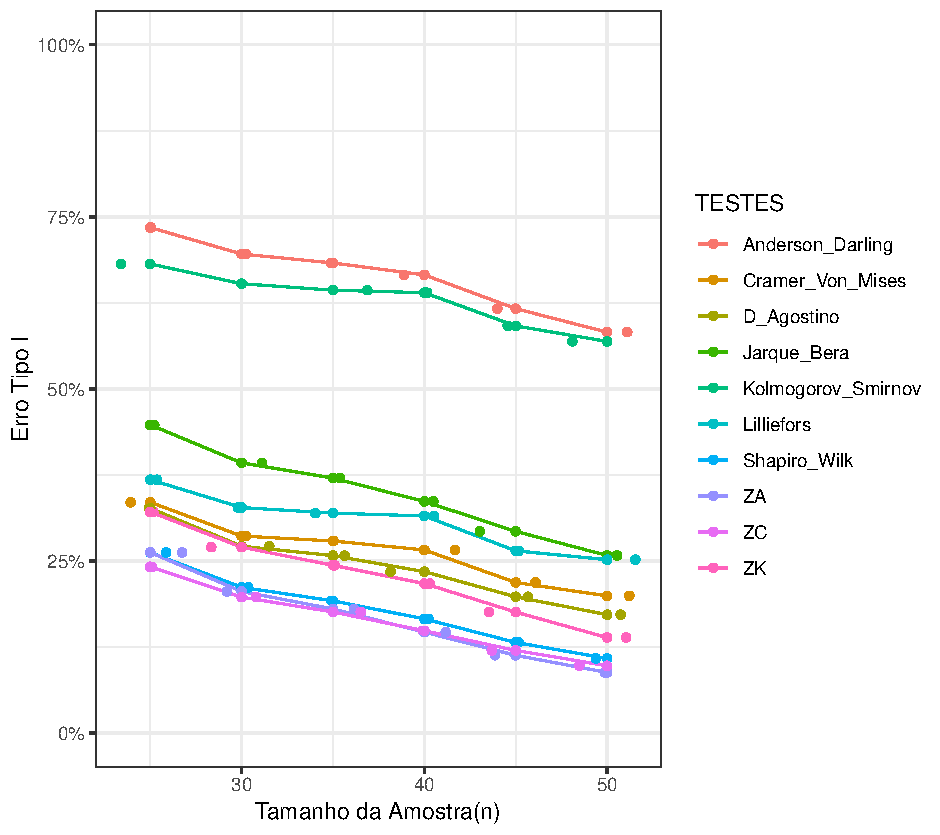
\includegraphics[width=\textwidth]{Distribuição_Beta/Erro_TipoI/erro_tipo_I_beta_50.pdf}
        \caption{\(N = 50\)}
        \label{fig:beta_50}
    \end{subfigure}
    \hfill
    % Terceira figura
    \begin{subfigure}[b]{0.32\textwidth}
        \centering
        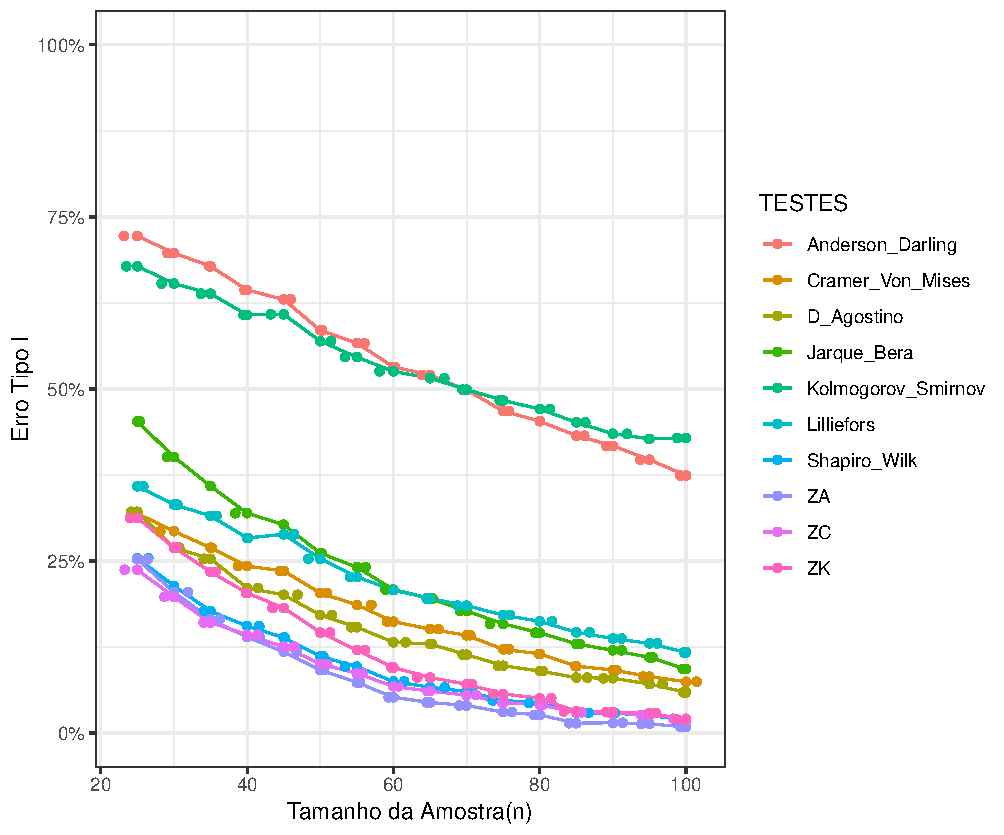
\includegraphics[width=\textwidth]{Distribuição_Beta/Erro_TipoI/erro_tipo_I_beta_100.pdf}
        \caption{\(N = 100\)}
        \label{fig:beta_100}
    \end{subfigure}
    \label{fig:erro_tipoI_beta}
\end{figure}



\begin{figure}[H]
    \centering
    % Primeira figura
    \begin{subfigure}[b]{0.33\textwidth}
        \centering
        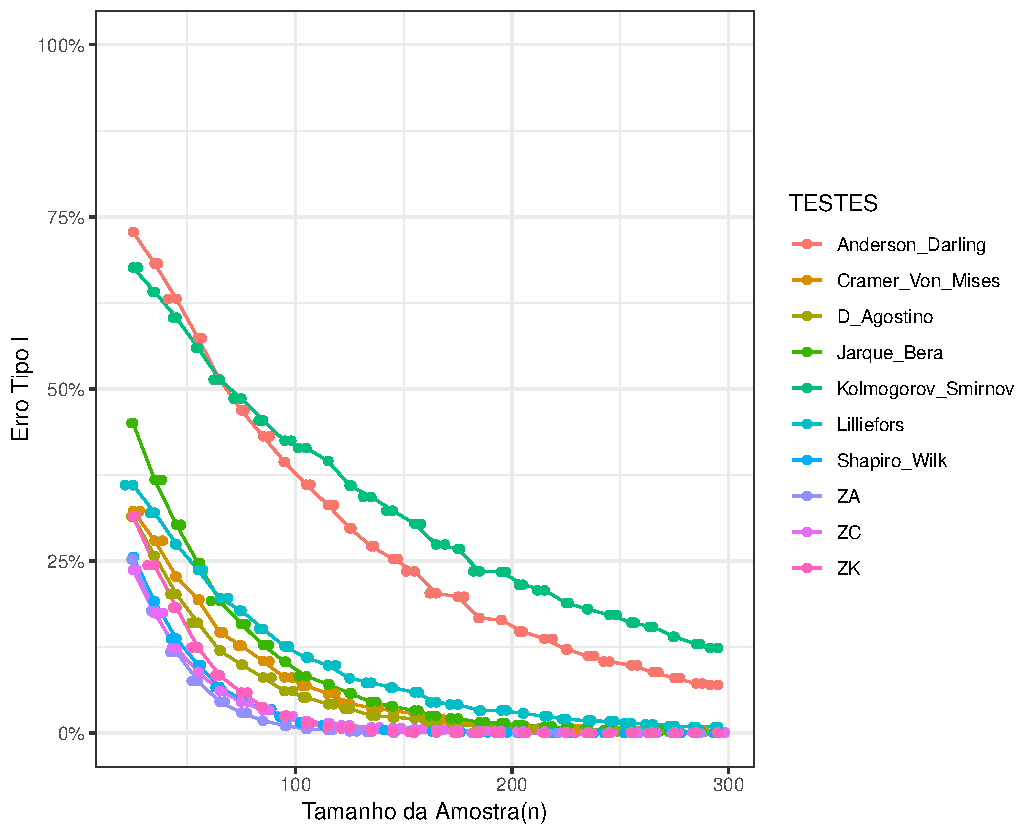
\includegraphics[width=\textwidth]{Distribuição_Beta/Erro_TipoI/erro_tipo_I_beta_300.pdf}
        \caption{\(N = 300\)}
        \label{fig:beta_30}
    \end{subfigure}
    \hfill
    % Segunda figura
    \begin{subfigure}[b]{0.33\textwidth}
        \centering
        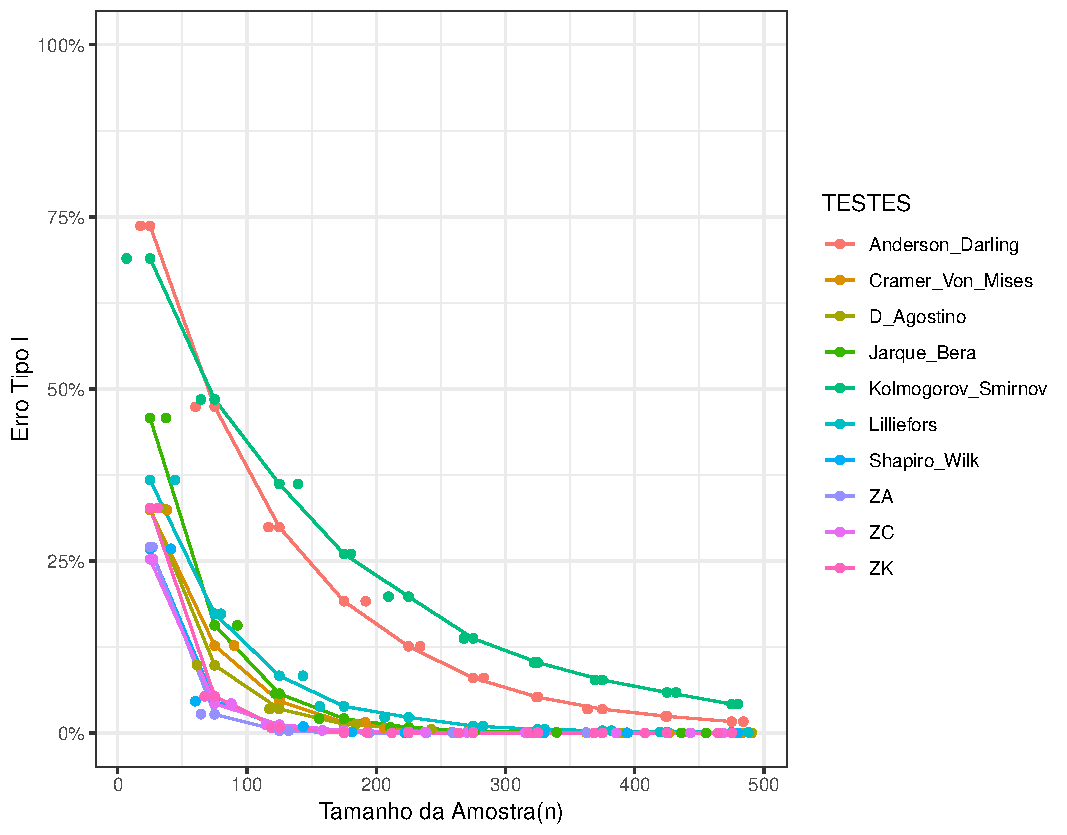
\includegraphics[width=\textwidth]{Distribuição_Beta/Erro_TipoI/erro_tipo_I_beta_500.pdf}
        \caption{\(N = 500\)}
        \label{fig:beta_50}
    \end{subfigure}
    \hfill
    % Terceira figura
    \begin{subfigure}[b]{0.29\textwidth}
        \centering
        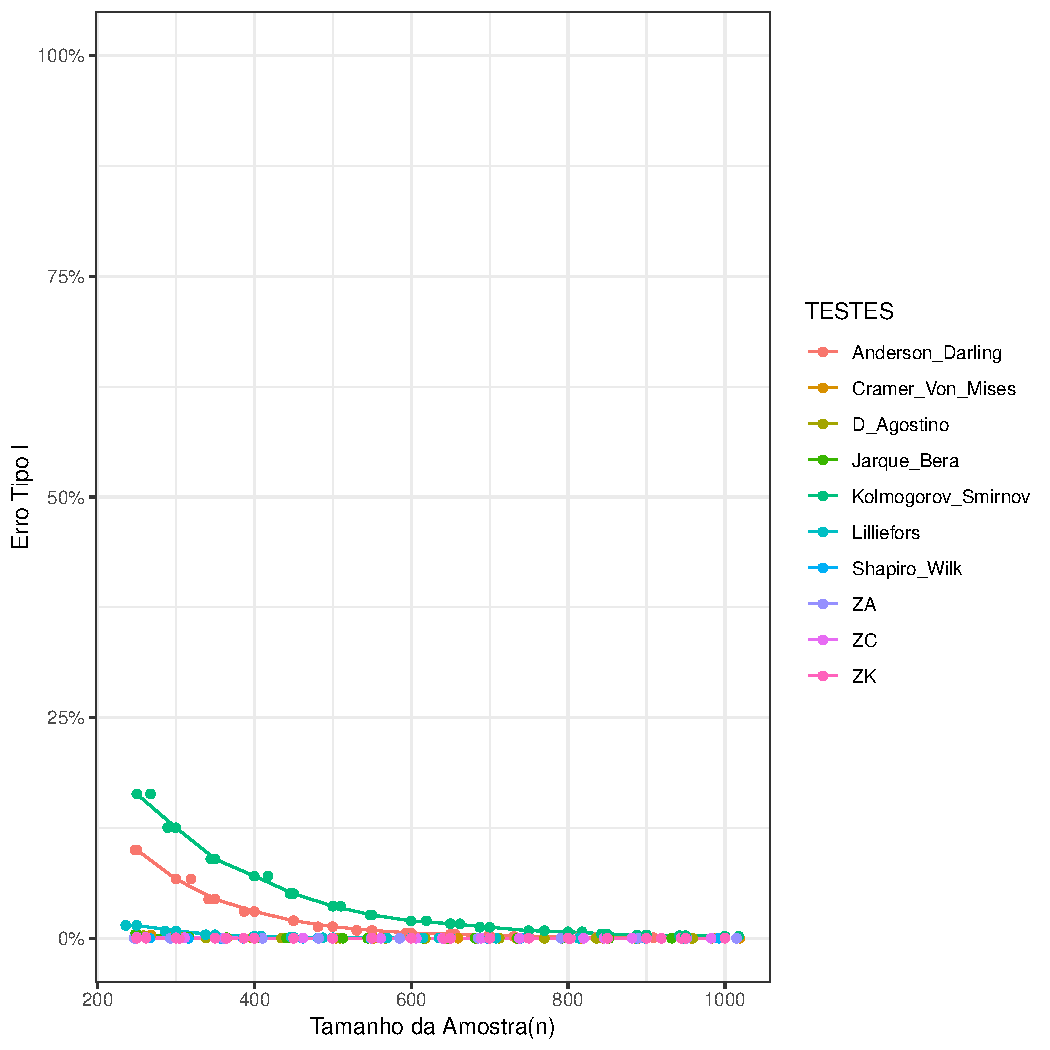
\includegraphics[width=\textwidth]{Distribuição_Beta/Erro_TipoI/erro_tipo_I_beta_1000.pdf}
        \caption{\(N = 1.000\)}
        \label{fig:beta_100}
    \end{subfigure}
    \label{fig:erro_tipoI_beta}
\end{figure}


%%%%%%%%%% Poder do Teste -> Distribuição Beta %%%%%%%%%%
\begin{figure}[H]
    \centering
      \caption{Comparação do Poder do Teste dos testes AD, CM, DG, LL, JB, KS, ZA, ZC e ZK em função do tamanho amostral para a \textbf{Distribuição} \(\textbf{Cauchy}(0, 1)\).}
    \label{fig:poder_teste_dist_cauchy}
    % Primeira figura
    \begin{subfigure}[b]{0.3\textwidth}
        \centering
        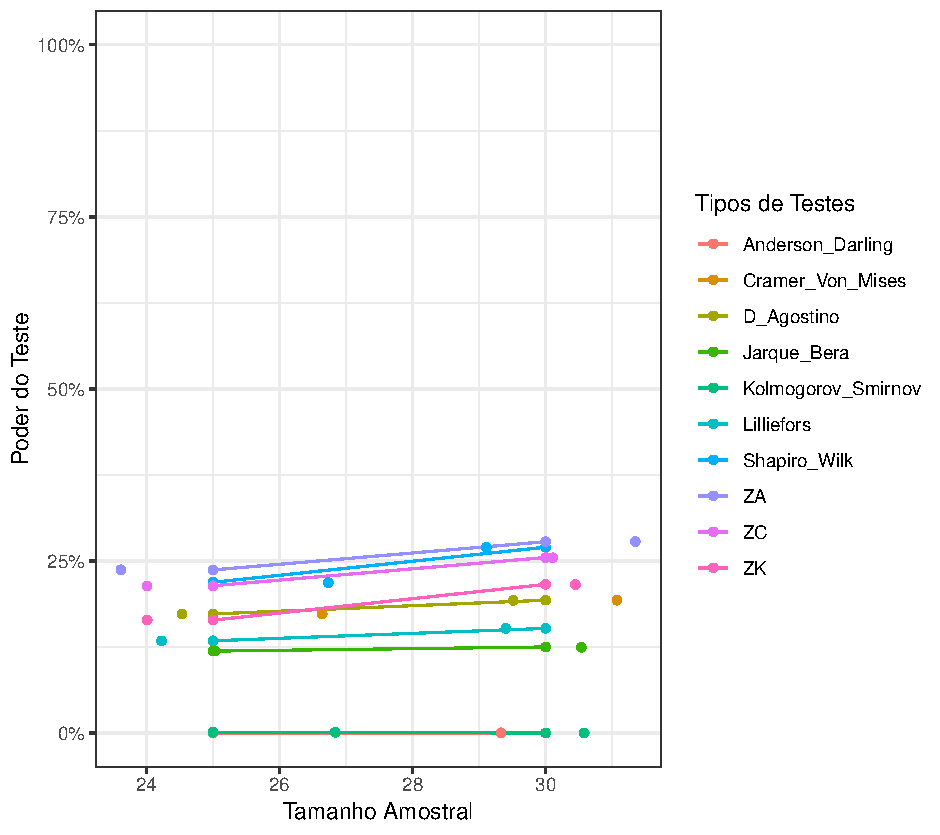
\includegraphics[width=\textwidth]{Distribuição_Beta/Poder_Teste/poder_teste_beta_30.pdf}
        \caption{(\(N = 30\)}
        \label{fig:beta_30}
    \end{subfigure}
    \hfill
    % Segunda figura
    \begin{subfigure}[b]{0.3\textwidth}
        \centering
        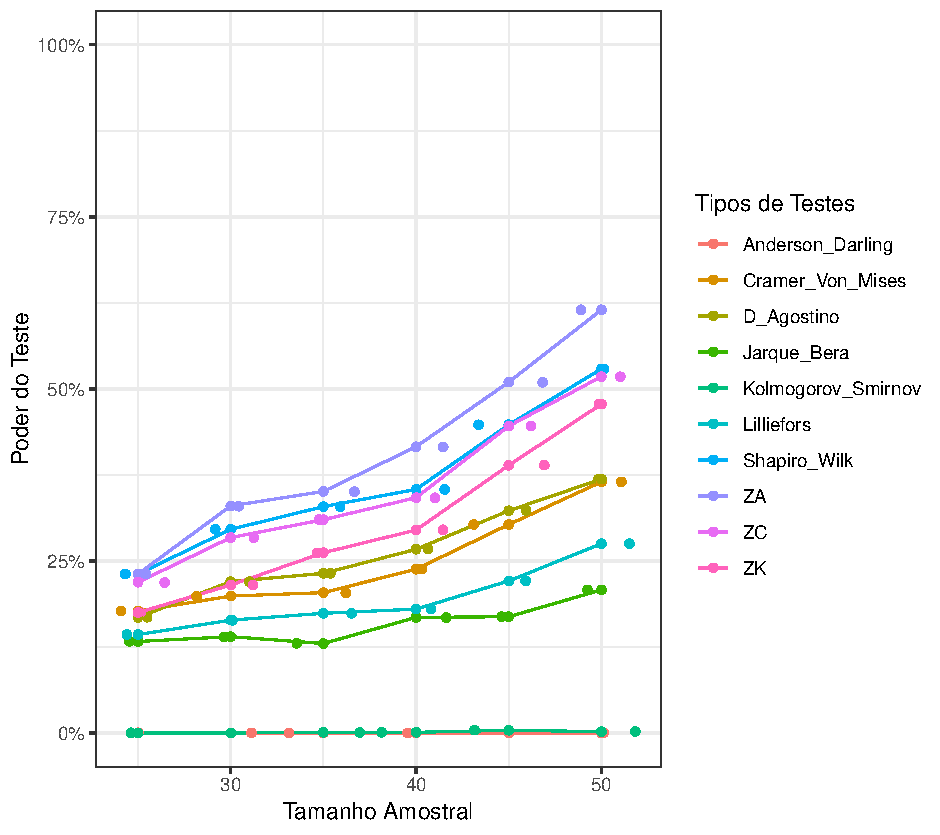
\includegraphics[width=\textwidth]{Distribuição_Beta/Poder_Teste/poder_teste_beta_50.pdf}
        \caption{\(N = 50\)}
        \label{fig:beta_50}
    \end{subfigure}
    \hfill
    % Terceira figura
    \begin{subfigure}[b]{0.32\textwidth}
        \centering
        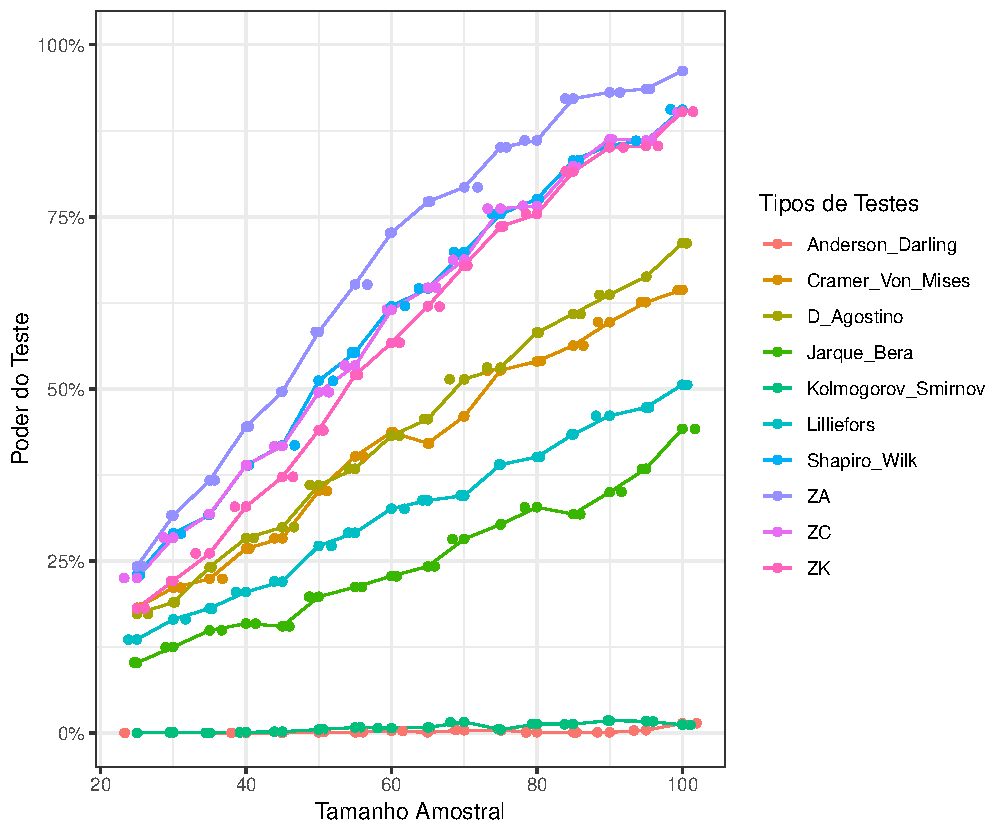
\includegraphics[width=\textwidth]{Distribuição_Beta/Poder_Teste/poder_teste_beta_100.pdf}
        \caption{\(N = 100\)}
        \label{fig:beta_100}
    \end{subfigure}
    \label{fig:erro_tipoI_beta}
\end{figure}






    
    


















    \vspace{1.3cm}
{\large\bfseries 5. REFERÊNCIAS}\par

    \vspace{1.3cm}

    
  
    \normalsize
  \end{column}
\end{columns}

\end{frame}
\end{document}
